% Options for packages loaded elsewhere
% Options for packages loaded elsewhere
\PassOptionsToPackage{unicode}{hyperref}
\PassOptionsToPackage{hyphens}{url}
\PassOptionsToPackage{dvipsnames,svgnames,x11names}{xcolor}
%
\documentclass[
  letterpaper,
  DIV=11,
  numbers=noendperiod]{scrartcl}
\usepackage{xcolor}
\usepackage{amsmath,amssymb}
\setcounter{secnumdepth}{5}
\usepackage{iftex}
\ifPDFTeX
  \usepackage[T1]{fontenc}
  \usepackage[utf8]{inputenc}
  \usepackage{textcomp} % provide euro and other symbols
\else % if luatex or xetex
  \usepackage{unicode-math} % this also loads fontspec
  \defaultfontfeatures{Scale=MatchLowercase}
  \defaultfontfeatures[\rmfamily]{Ligatures=TeX,Scale=1}
\fi
\usepackage{lmodern}
\ifPDFTeX\else
  % xetex/luatex font selection
\fi
% Use upquote if available, for straight quotes in verbatim environments
\IfFileExists{upquote.sty}{\usepackage{upquote}}{}
\IfFileExists{microtype.sty}{% use microtype if available
  \usepackage[]{microtype}
  \UseMicrotypeSet[protrusion]{basicmath} % disable protrusion for tt fonts
}{}
\makeatletter
\@ifundefined{KOMAClassName}{% if non-KOMA class
  \IfFileExists{parskip.sty}{%
    \usepackage{parskip}
  }{% else
    \setlength{\parindent}{0pt}
    \setlength{\parskip}{6pt plus 2pt minus 1pt}}
}{% if KOMA class
  \KOMAoptions{parskip=half}}
\makeatother
% Make \paragraph and \subparagraph free-standing
\makeatletter
\ifx\paragraph\undefined\else
  \let\oldparagraph\paragraph
  \renewcommand{\paragraph}{
    \@ifstar
      \xxxParagraphStar
      \xxxParagraphNoStar
  }
  \newcommand{\xxxParagraphStar}[1]{\oldparagraph*{#1}\mbox{}}
  \newcommand{\xxxParagraphNoStar}[1]{\oldparagraph{#1}\mbox{}}
\fi
\ifx\subparagraph\undefined\else
  \let\oldsubparagraph\subparagraph
  \renewcommand{\subparagraph}{
    \@ifstar
      \xxxSubParagraphStar
      \xxxSubParagraphNoStar
  }
  \newcommand{\xxxSubParagraphStar}[1]{\oldsubparagraph*{#1}\mbox{}}
  \newcommand{\xxxSubParagraphNoStar}[1]{\oldsubparagraph{#1}\mbox{}}
\fi
\makeatother


\usepackage{longtable,booktabs,array}
\usepackage{calc} % for calculating minipage widths
% Correct order of tables after \paragraph or \subparagraph
\usepackage{etoolbox}
\makeatletter
\patchcmd\longtable{\par}{\if@noskipsec\mbox{}\fi\par}{}{}
\makeatother
% Allow footnotes in longtable head/foot
\IfFileExists{footnotehyper.sty}{\usepackage{footnotehyper}}{\usepackage{footnote}}
\makesavenoteenv{longtable}
\usepackage{graphicx}
\makeatletter
\newsavebox\pandoc@box
\newcommand*\pandocbounded[1]{% scales image to fit in text height/width
  \sbox\pandoc@box{#1}%
  \Gscale@div\@tempa{\textheight}{\dimexpr\ht\pandoc@box+\dp\pandoc@box\relax}%
  \Gscale@div\@tempb{\linewidth}{\wd\pandoc@box}%
  \ifdim\@tempb\p@<\@tempa\p@\let\@tempa\@tempb\fi% select the smaller of both
  \ifdim\@tempa\p@<\p@\scalebox{\@tempa}{\usebox\pandoc@box}%
  \else\usebox{\pandoc@box}%
  \fi%
}
% Set default figure placement to htbp
\def\fps@figure{htbp}
\makeatother





\setlength{\emergencystretch}{3em} % prevent overfull lines

\providecommand{\tightlist}{%
  \setlength{\itemsep}{0pt}\setlength{\parskip}{0pt}}



 


\KOMAoption{captions}{tableheading}
\makeatletter
\@ifpackageloaded{caption}{}{\usepackage{caption}}
\AtBeginDocument{%
\ifdefined\contentsname
  \renewcommand*\contentsname{Table of contents}
\else
  \newcommand\contentsname{Table of contents}
\fi
\ifdefined\listfigurename
  \renewcommand*\listfigurename{List of Figures}
\else
  \newcommand\listfigurename{List of Figures}
\fi
\ifdefined\listtablename
  \renewcommand*\listtablename{List of Tables}
\else
  \newcommand\listtablename{List of Tables}
\fi
\ifdefined\figurename
  \renewcommand*\figurename{Figure}
\else
  \newcommand\figurename{Figure}
\fi
\ifdefined\tablename
  \renewcommand*\tablename{Table}
\else
  \newcommand\tablename{Table}
\fi
}
\@ifpackageloaded{float}{}{\usepackage{float}}
\floatstyle{ruled}
\@ifundefined{c@chapter}{\newfloat{codelisting}{h}{lop}}{\newfloat{codelisting}{h}{lop}[chapter]}
\floatname{codelisting}{Listing}
\newcommand*\listoflistings{\listof{codelisting}{List of Listings}}
\makeatother
\makeatletter
\makeatother
\makeatletter
\@ifpackageloaded{caption}{}{\usepackage{caption}}
\@ifpackageloaded{subcaption}{}{\usepackage{subcaption}}
\makeatother
\usepackage{bookmark}
\IfFileExists{xurl.sty}{\usepackage{xurl}}{} % add URL line breaks if available
\urlstyle{same}
\hypersetup{
  pdftitle={Fear alone influences the behaviour of a keystone native prey by an invader; a non-consumptive effect of the catfish invasion of Aotearoa New Zealand's freshwaters},
  pdfauthor={Olivier V. Raven; Calum MacNeil; Finnbar Lee; Robin Holmes; Ian A. Kusabs; Francis J. Burdon; Deniz Özkundakci},
  pdfkeywords={Non-consumptive effects, crayfish, catfish
invasion, kōura, longfin eel},
  colorlinks=true,
  linkcolor={blue},
  filecolor={Maroon},
  citecolor={Blue},
  urlcolor={Blue},
  pdfcreator={LaTeX via pandoc}}


\title{Fear alone influences the behaviour of a keystone native prey by
an invader; a non-consumptive effect of the catfish invasion of Aotearoa
New Zealand's freshwaters}
\author{Olivier V. Raven \and Calum MacNeil \and Finnbar Lee \and Robin
Holmes \and Ian A. Kusabs \and Francis J. Burdon \and Deniz Özkundakci}
\date{2026-03-30}
\begin{document}
\maketitle
\begin{abstract}
Non-consumptive effects (NCEs) or `fear' responses to predators
encompass costly antipredator behaviours, such as increasing refuge use
in conjunction with decreasing foraging and feeding efficiency. Such
NCEs could influence prey population dynamics and even community
structure and function, if the prey themselves are `keystone' species.
In Aotearoa-New Zealand, the native freshwater crayfish kōura
(\emph{Paranephrops planifrons}) is a keystone species and an ecosystem
engineer but is preyed upon by native longfin eels (\emph{Anguilla
dieffenbachii}) and invasive brown bullhead catfish (\emph{Ameiurus
nebulosus}). Using controlled aquarium experiments, we tested whether
visual and chemical cues from each predator induced changes in kōura
refuge-seeking and feeding behaviour. Neither predator treatment
significantly affected refuge use or feeding rate. The absence of a
significant response to either predator, including the co-evolved eel,
may reflect limited prior predator experience in the source lakes where
eel densities are low. Substantial individual variation in kōura
behaviour further reduced statistical power to detect treatment effects,
highlighting the importance of accounting for personality differences in
future NCE studies.
\end{abstract}

\renewcommand*\contentsname{Table of contents}
{
\hypersetup{linkcolor=}
\setcounter{tocdepth}{3}
\tableofcontents
}

\section{Introduction}\label{introduction}

Biological invasions can have profound impacts on invaded ecosystems,
particularly through the introduction of novel predators that prey upon
native species lacking an evolutionary history with them (Doherty et
al., 2016). Native prey are often naïve to these predators, making them
especially vulnerable to direct predation (Gamradt \& Kats, 1996; Smith
et al., 2008). In addition to these consumptive effects (CEs), native
prey may exhibit heightened fear responses to invasive predators,
leading to the development of anti-predator behaviours such as increased
refuge use and avoidance of open habitats (Kindlinger \& Albins, 2017).
These behavioural changes, termed non-consumptive effects (NCEs), can
substantially influence population dynamics by reducing foraging
activity, growth, and reproductive output (Pressier et al., 2005). In
contrast, native predators generally elicit different responses because
prey and predators have co-evolved, resulting in behavioural and
physiological adaptations that stabilise predator--prey interactions
within local ecosystems (Abrams, 2000).

Freshwater crayfish rely primarily on chemical cues (kairomones) rather
than visual cues to detect and respond to predatory fish (Blake \& Hart,
1993; Brönmark \& Hansson, 2012). The kairomones carry signals via
excreta, mucus, or skin, that crayfish use to assess predator risk,
responding more strongly to predators that have consumed conspecifics
and to alarm cues released when prey are injured or killed (Gherardi et
al., 2011; Beattie \& Moore, 2018). Exposure to kairomones from
predatory fish can generate NCEs, including reduced growth and reduced
activity levels in crayfish (Adams, 2007; Ramberg-Pihl \& Yurewicz,
2020), and even non-predatory fish can cause these behaviour changes,
likely through heightened generalised awareness of risk (Nyström, 2005).
However, the strength of these responses depends on prior experience as
wild-caught individual crayfish show stronger antipredator responses
than farmed conspecifics naive to predators (Martin, 2014), indicating
that both individual experiences and evolutionary history shape
kairomones detection.

In Aotearoa-New Zealand (hereafter Aotearoa), the endemic northern
freshwater crayfish \emph{Paranephrops planifrons} White, 1842 commonly
known as kōura is a `culturally treasured' taonga species and valued
food resource for Māori the indigenous people of Aotearoa (Kusabs \&
Quinn, 2009). Ecologically, kōura play a critical role in freshwater
ecosystems as ecosystem engineers through their effects on sediment
dynamics, nutrient cycling, and benthic community structure, and have
been described as keystone species in many freshwater systems (Collier
at al., 1997; Parkyn et al., 2001; Usio \& Townsend, 2004). Kōura have a
long co-evolutionary history with the native longfin eel (\emph{Anguilla
dieffenbachii}) and shortfin eel (\emph{A. australis}) (MacNeil et al.,
2025) and have been shown to respond more strongly to eel kairomones
than to those of introduced non-native brown trout (\emph{Salmo
trutta}), even when sourced from streams where trout are present (Shave
et al., 1994). This suggests that co-evolutionary history, rather than
individual experience alone, shapes kōura predator recognition (Shave et
al., 1994). Currently kōura are threatened by multiple interacting
stressors, including climate change, water-quality degradation and
invasive species, contributing to widespread population declines (Lee et
al., 2025; Kusabs et al., in revision). One of the invasive species that
threatens the kōura is the non-native brown bullhead catfish
(\emph{Ameiurus nebulosus}; Barnes \& Hicks, 2003; Dedual, 2019), which
has been introduced in Aotearoa in 1878 and has spread over various
waterways on the North Island (McDowall, 1990; Lee et al., 2025). The
brown bullhead catfish is highly tolerant of a wide range of
environmental conditions (Lee et al., 2025) and, due to its broad gape
and opportunistic feeding behaviour, is capable of consuming a wide
variety of native aquatic organisms (Scott \& Crossman, 1973; Dedual,
2019). The recent and ongoing spread of brown bullhead catfish into
North Island waterways therefore represents a novel predation threat to
which kōura may lack adequate behavioural or sensory adaptations.

In this study, controlled aquarium experiments were used to test whether
predator presence and associated chemical cues induce changes in
refuge-seeking and feeding behaviour, providing insight into the
behavioural mechanisms underlying NCEs of kōura responses to native and
invasive predation threats. It is expected that kōura would show more
shelter-seeking behaviour when presented with eels compared to catfish,
due to naivety of the kōura towards catfish. Also, it is expected that
light regime would have an influence on shelter seeking behaviour of
this nocturnal species. For feeding behaviour it is expected that kōura
will feed less when exposed to eel kairomones but as they will be naïve
to catfish kairomones, feeding will be similar to the control. The
findings of this study contribute to understanding the behavioural
mechanisms underlying kōura vulnerability to invasive catfish and
provide a basis for predicting population-level impacts as catfish
continue to spread into uninvaded waterways across Aotearoa.

\section{Materials and Methods}\label{materials-and-methods}

\subsection{Animal collection and
preparation}\label{animal-collection-and-preparation}

On August 19th, 2025, kōura were sourced from two catfish-free lakes,
(Ōkāreka and Tikitapu (Blue Lake)) in the Rotorua Te Awara Lakes area,
Bay of Plenty region of the North Island. On September 25th, 2025, Brown
bullhead catfish and longfin eels were sourced from Lake Rotoroa in
Hamilton in the Waikato region of the North Island. Experiments were
conducted at the Aquatic Research Centre of the University of Waikato.
Some kōura were previously used in a mesocosm habitat preference study
but never exposed to a predator. They were acclimated for a week in
holding tanks under controlled conditions: a 10:14 light: dark cycle
reflecting the correct seasonal day-length at a stable temperature of
15.6 °C, pH 8.4 and 10 mg l⁻¹ dissolved oxygen. Kōura were fed every
other day fish food pellets (Hikari Tropical carnivore pellets, animal
protein 47\%). Catfish and eels were held in separate holding tanks,
with the same environmental and feeding regime to kōura.

Because kōura are taonga (culturally important) species, permission had
to be sought from relevant iwi (Māori tribal unit), as well as relevant
government regulator to source a limited number of animals. Experiments
were adapted, particularly the feeding study to make the best use of the
finite number of collected animals. As this study focused on kōura the
catfish and eels were reused repeatedly in the study.

\subsection{Refuge experiment}\label{refuge-experiment}

Prior to the experiments, all animals were individually weighed and
measured. Only male kōura were used. Kōura had a mean (± SD) orbital
carapace length (OCL) of 26.0 mm (± 3.08) (18.35-32.95 mm range) and a
mean wet weight of 11.7 g (± 4.25) (3--23 g range). Catfish ranged in
length from 260-267 mm and 2.34 -- 3.16 kg wet weight and eels ranged in
length from ? and 2.50-3.52 kg wet weight.

Experiments were conducted in 38 L glass tanks (600 × 200 × 220 mm) with
each tank having three sides (apart from front of tank) blacked out to
block visual cues from neighbouring tanks. Each tank was divided into
two compartments by a 0.5 mm steel mesh divider, allowing visual and
chemical cues between compartments, while preventing physical contact
between animals on either side of barrier
(Figure~\ref{fig-aquarium-setup}). All tanks were filled with 26.4 L
dechlorinated tap water and had identical environmental regimes as
previously detailed for acclimatisation tanks, with water flow provided
by an air stone lodged the top of the barrier in each tank. Each tank
housed a single kōura on one side of the barrier and either a single
predator (catfish or eel) or no predator (control) on the other side. A
halved terracotta pot (90 mm diameter × 90 mm depth) was positioned on
the kōura side of the tank to serve as a potential refuge. To control
for potential tank or side effects, the position of predator treatments
within the aquaria was systematically rotated between experimental
rounds. The experiment was repeated across five rounds, resulting in 11
catfish replicates, 11 eel replicates, and 10 control replicates. This
experiment was first carried out in the light (n = 32 tanks) before
being repeated in the dark (n = 32 tanks) with a total of 64 tanks used.
Observations were made in the dark using red lighting positioned above
the tanks in the same location as the previous normal lighting for the
light regime observations. Following each individual experimental run,
each tank was thoroughly cleaned and refilled with dechlorinated tap
water before reuse. Each individual kōura was only exposed once to a
fish predator and there were no mortalities of kōura or fish during the
course of experiments. All experiments were conducted within a
three-week period (from 1/10/2025 to 16/10/2025), the dark trials
following on from the light trials.

Observations of each kōura location was made 21 times at the following
time intervals (in minutes): 0, 5, 10, 20, 30, 45, 60, 61, 65, 70, 80,
90, 120, 150, 210, 240, 245, 260, 275, 290, and 300. An individual kōura
were placed in the middle of the tank compartment containing the refuge
at 0-minute (its initial location being immediately noted after its
addition to the tank) and was removed after the final 300-minute
observation. The fish predator was introduced after 60 minutes into the
tank on the other side of the barrier from the kōura compartment and
removed again at 240 minutes. The control tanks had no fish added but at
60 minutes and again at 240 minutes the water in the `predator'
compartment was disturbed by mixing with a small net for approximately
30 seconds. This was to simulate the disturbance time associated with
adding and removing fish in the other treatments. Kōura location within
each tank was recorded at each time interval as either refuge (the
animal was using the refuge, being inside it or immediately behind it
and touching it) or in the open - non-refuge (any other location in the
tank where the animal was not in the refuge or touching the refuge).

\subsection{Feeding experiment}\label{feeding-experiment}

The feeding behaviour experiments were executed in 16 glass tanks of
9.25L (320 × 170 × 170 mm) filled with 5 L dechlorinated tap water and a
halved terracotta pot (90 mm diameter × 90 mm depth). In three rounds a
total of 46 male and two female kōura were placed individually in each
tank. Kōura had a mean (± SD) orbital carapace length (OCL) of 27.84 mm
(± 4.72) (20.48-41.15 mm range) and a mean wet weight of 15.65 g (±
8.84) (6-44 g range). For each round kōura were starved for different
periods (0, 3 and 4 days) prior to the feeding experiment to also
investigate how starvation period influenced feeding motivation.

Kairomones from catfish and eels were collected by placing 4 fish
(catfish or eel) in a 10 L bucket filled with water from the holding
tanks for 15 minutes to concentrate the kairomones in the water. 1 L
from the buckets was added to the tank with the kōura in it and for the
controls 1 L of dechlorinated tap water was added. Next, 10 Hikari
Tropical carnivore pellets were added to each tank. After 24 hours, when
each experiment terminated, the number of pellets eaten (to the nearest
quarter pellet) was counted and the feeding rate (pellets consumed per g
kōura) calculated. As stated previously, the feeding study was adapted
to make the best use of the finite number of collected taonga animals
and the following protocols reflect this. After 0 days starvation, 16
kōura (14 male and 2 female) were exposed to eel water (n = 5), catfish
water (n = 6) or control water (n = 5). After 3 days starvation, 16
kōura (male only) were exposed to eel water (n = 6), catfish water (n =
5) or control water (n = 5). After 4 days starvation, 16 kōura (male
only) were exposed to eel water (n = 5), catfish water (n = 5) or
control water (n = 6).

\subsection{Data analysis}\label{data-analysis}

To analyse kōura refuge use a beta-binomial generalized linear
mixed-effects model (GLMM; BRON) fitted using the glmmTMB package in R
(BRON; BRON). The response variable was the number of observations in
refuge out of total observations per experiment round, treatment
(catfish/eel/control), light condition (light, dark), period
(before/during/after) included as fixed effects. A beta-binomial
distribution was used to account for overdispersion in the binomial
proportion data. Model selection was conducted by comparing candidate
models differing in fixed effect structure and random effect inclusion
using AIC, with the model with the lowest AIC selected as optimal. The
need for a tank-level random intercept was evaluated by comparing AIC
between models with and without this term. Model fit of the final model
was assessed using DHARMa simulation-based residuals, including tests
for overdispersion and zero-inflation (Hartig et al., 2024). Marginal
means and pairwise contrasts between factor levels were obtained using
the emmeans package (Lenth et al., 2026).

The feeding rate was analysed using a linear model with pellets consumed
per gram body weight as the response, and treatment (catfish, eel,
control) and starvation period (0, 3, 4) as fixed effects, including
their interaction. Because each starvation period was conducted in a
separate experimental round, starvation period and round were fully
confounded by design, precluding the inclusion of round as a random
effect. Overall significance of fixed effects was assessed using Type
III ANOVA (car package; Fox \& Weisberg, 2018), and model assumptions
were verified using residual plots and testing normality of residuals
using the Shapiro-Wilk test. Pairwise comparisons between treatment and
starvation level combinations were conducted using estimated marginal.

\section{Results}\label{results}

\subsection{Refuge experiment}\label{refuge-experiment-1}

The proportion of time kōura spent in refuge varied across treatments,
experimental periods, and light conditions
(Figure~\ref{fig-refuge-plot}, Table~\ref{tbl-s1-refuge-prop}). Under
dark conditions, refuge use increased across the experimental period in
the catfish treatment, rising from 0.39 before to 0.7 after exposure,
while the control showed a smaller increase (0.37 to 0.47) and
eel-exposed kōura showed little change (0.27 before, 0.41 during, and
0.36 after). Under light conditions, refuge use was generally higher
than under dark conditions, with catfish (0.52 before to 0.73 after) and
control (0.4 to 0.82) both showing increases across periods, while
eel-exposed kōura showed a smaller increase (0.35 to 0.53).

A beta-binomial GLMM with experimental unit as a random intercept was
the best supported model (lowest AIC). Full model coefficients are
reported in Table~\ref{tbl-s2-fixed-effects}. Refuge use was most
affected by period with more kōura using the refuge as the experiment
progressed. Refuge use was significantly more in the during period than
in the before period (\emph{p} = 0.144, Figure~\ref{fig-emmeans-plot},
Table~\ref{tbl-s3-emmeans}). This was also the case between before and
after period (\emph{p} = 0.007), but not between during and after
(\emph{p} = 0.409). Neither treatment nor light condition significantly
affected refuge use. No significant differences were found between
catfish and eel (\emph{p} = 0.01), catfish and control (\emph{p} = ), or
control and eel (\emph{p} = 0.314). Light condition was also not
significant (\emph{p} = ).

\subsection{Feeding experiment}\label{feeding-experiment-1}

The feeding experiment showed the highest mean (±SE) feeding rate was
after 3 days of starvation in the catfish treatment (0.235 ± 0.037
pellets g⁻¹). The linear model showed starvation period had significant
effect on feeding rate (\emph{p} = \ensuremath{4\times 10^{-4}},
Table~\ref{tbl-s4-feeding-anova}). Treatment had no significant effect
on feeding rate (\emph{p} = 0.968), and the interaction between the
treatment and starvation period was not significant (\emph{p} = 0.082),
although a marginal trend was observed (Figure~\ref{fig-feeding-plot}).
No significant difference was found in feeding rate between catfish,
eel, and control treatments within each of the starvation periods, this
suggests that predator kairomones did not affect feeding behaviour in
kōura within this experiment.

\section{Discussion}\label{discussion}

\subsection{Refuge experiment}\label{refuge-experiment-2}

\subsection{Feeding experiment}\label{feeding-experiment-2}

\subsection{Conclusion}\label{conclusion}

\section*{Acknowledgements}\label{acknowledgements}
\addcontentsline{toc}{section}{Acknowledgements}

\section*{References}\label{references}
\addcontentsline{toc}{section}{References}

\section*{Tables}\label{tables}
\addcontentsline{toc}{section}{Tables}

\section*{Figures}\label{figures}
\addcontentsline{toc}{section}{Figures}

\begin{figure}

\centering{

\pandocbounded{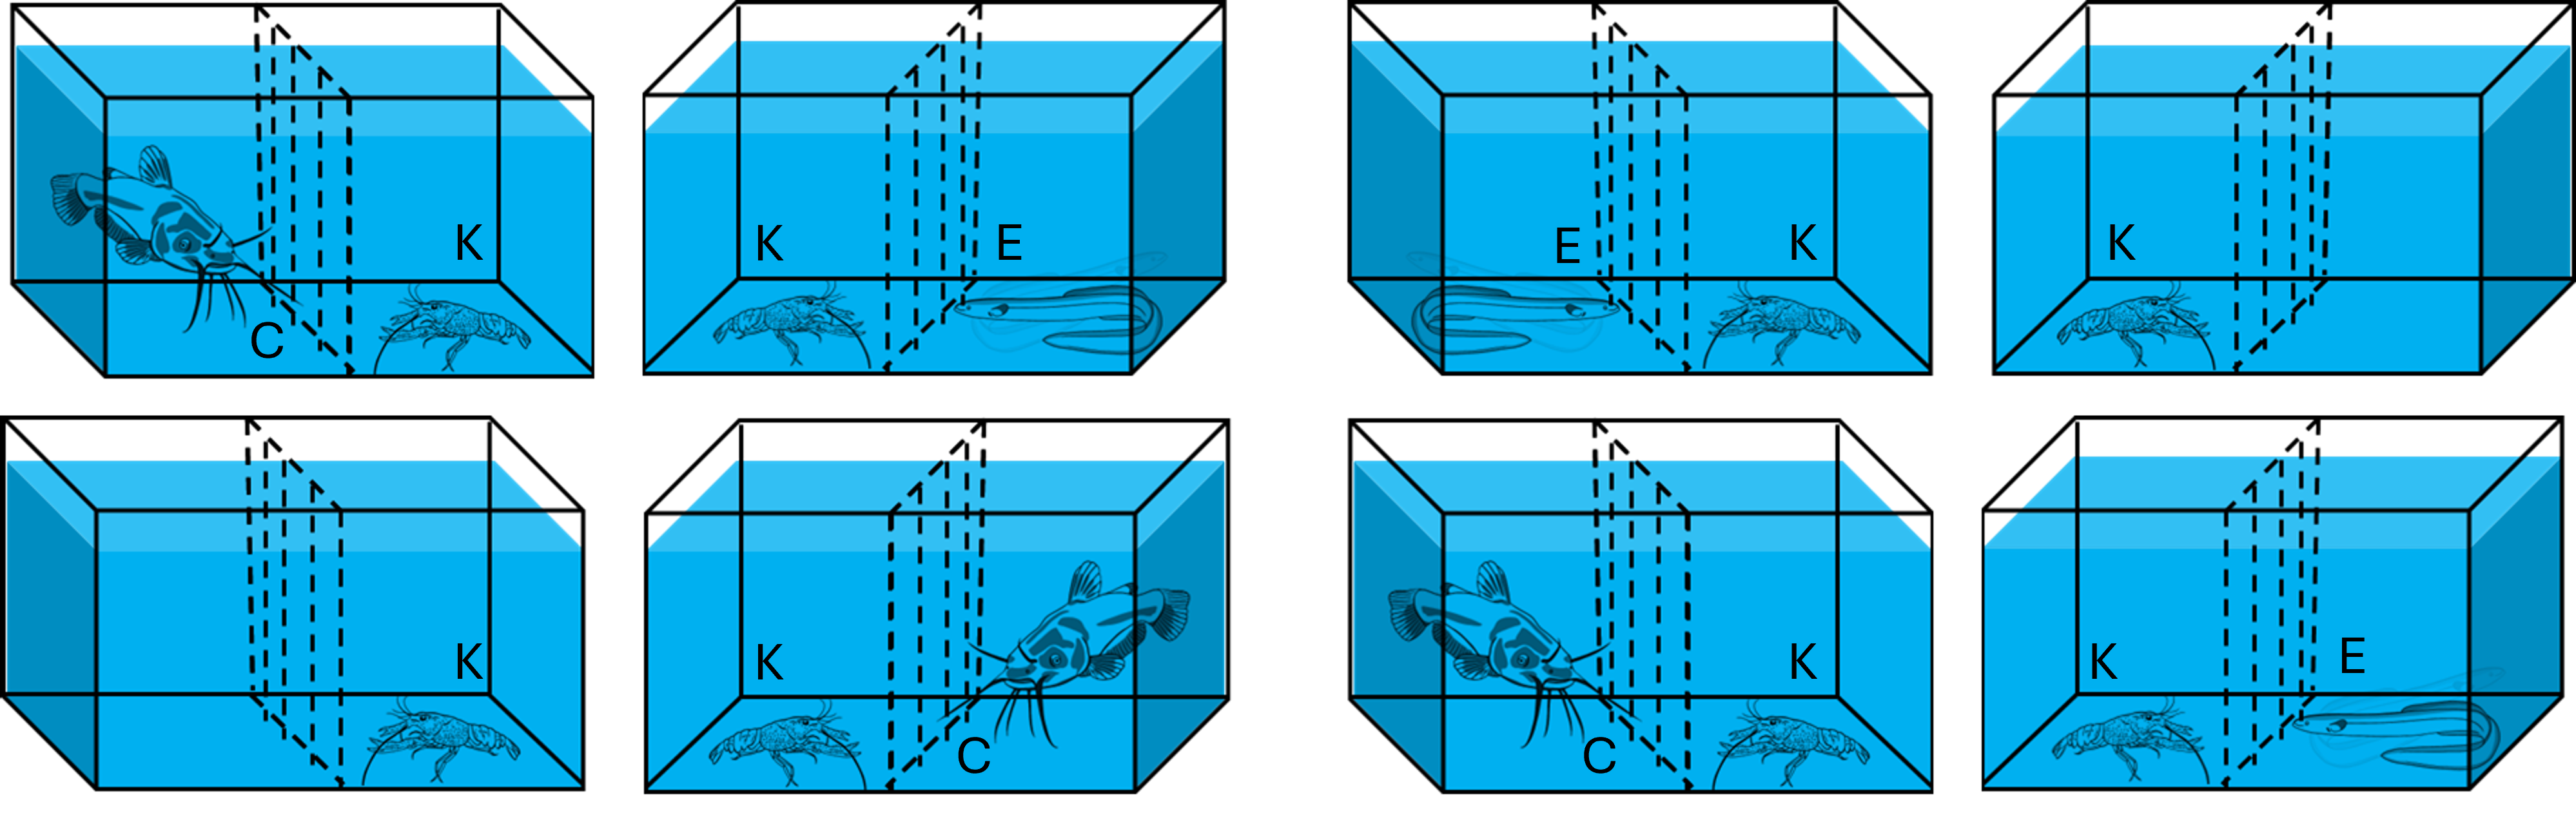
\includegraphics[keepaspectratio]{images/aquarium_setup.png}}

}

\caption{\label{fig-aquarium-setup}Schematic overview of the
experimental aquarium layout for one experimental round. Eight aquaria
were run simultaneously. In each tank, a single kōura (K) was housed on
one side of the aquarium with a shelter, while a predator (catfish (C)
or eel (E)) or no predator (control) was placed on the opposite side
behind a mesh divider allowing visual and chemical cues but preventing
physical contact.}

\end{figure}%

\begin{verbatim}
systemfonts and textshaping have been compiled with different versions of Freetype. Because of this, textshaping will not use the font cache provided by systemfonts
\end{verbatim}

\begin{figure}[H]

\centering{

\pandocbounded{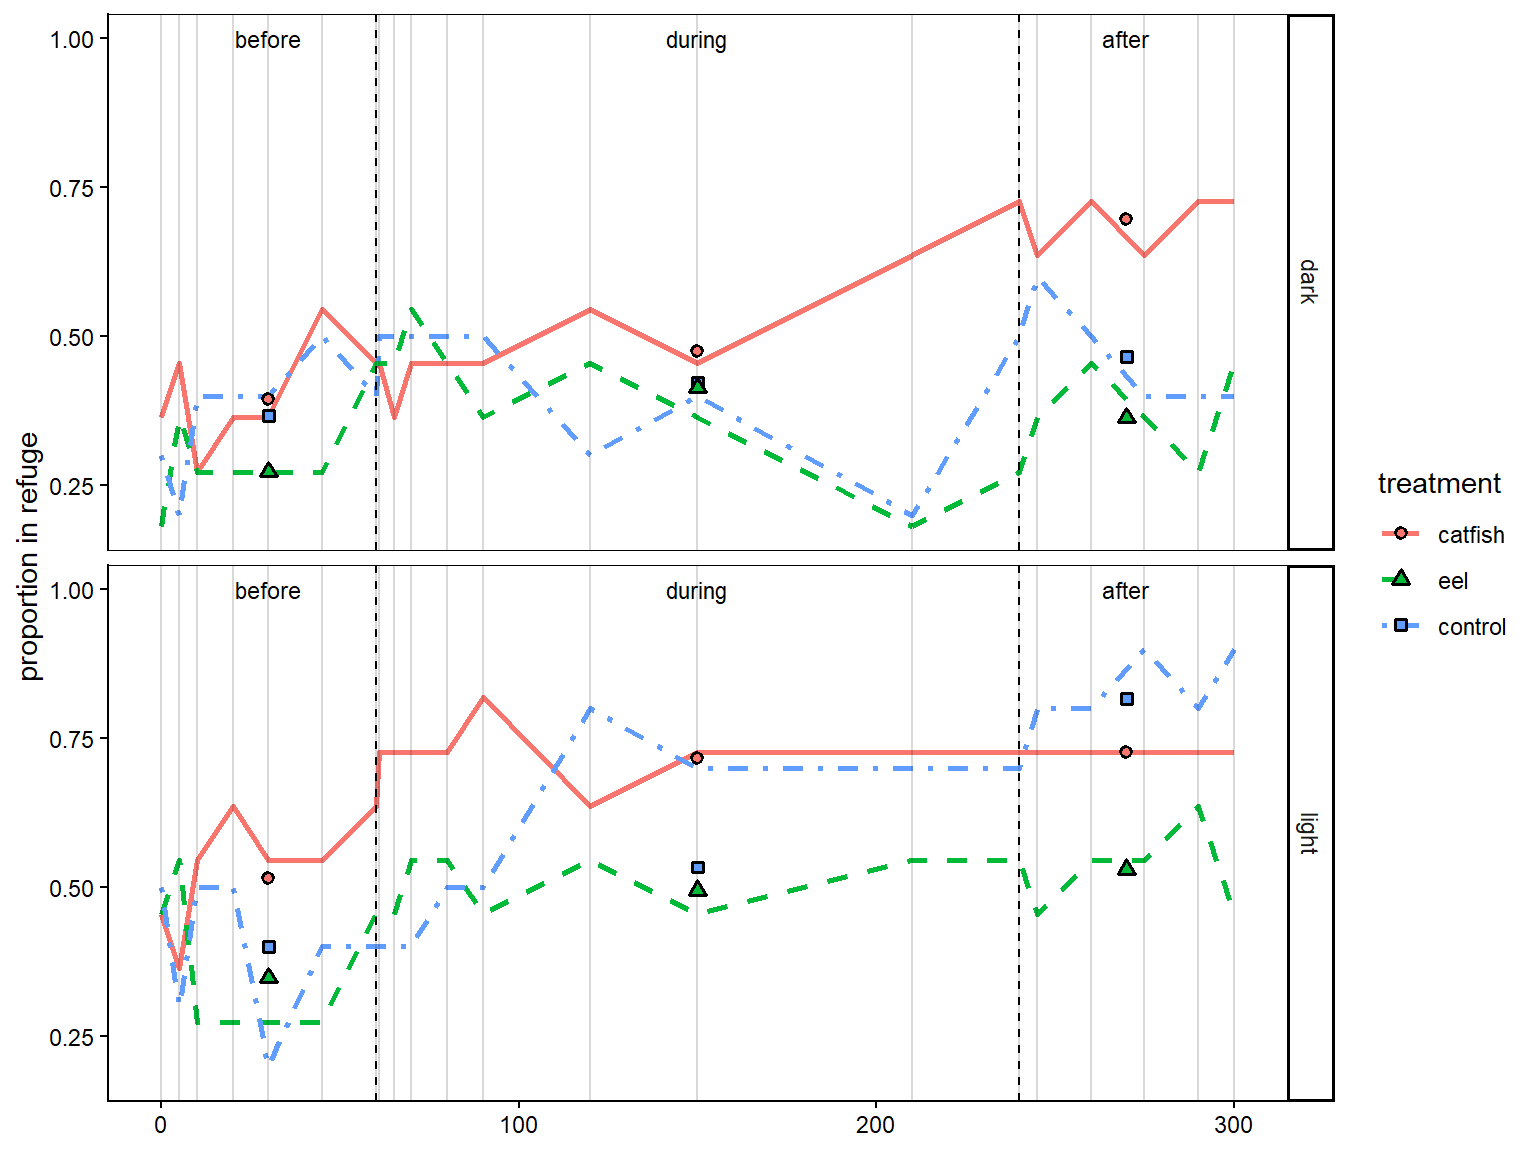
\includegraphics[keepaspectratio]{index_files/figure-latex/analysis-fig-refuge-plot-output-2.png}}

}

\caption{\label{fig-refuge-plot}Kōura use of refuge over course of
experiment with the three periods (before, during, after), the treatment
(catfish; red-solid circle, eel; green-dashed triangle, control;
blue-dotdash square), and divided over light regime (combined, dark,
light). The points represent the proportion within each period for each
treatment.}

\end{figure}%

\textsubscript{Source:
\href{https://OlivierRaven.github.io/https---github.com-OlivierRaven-NCE_Koura_catfish/analysis-preview.html\#cell-fig-refuge-plot}{Analysis
Notebook}}

\begin{figure}[H]

\centering{

\pandocbounded{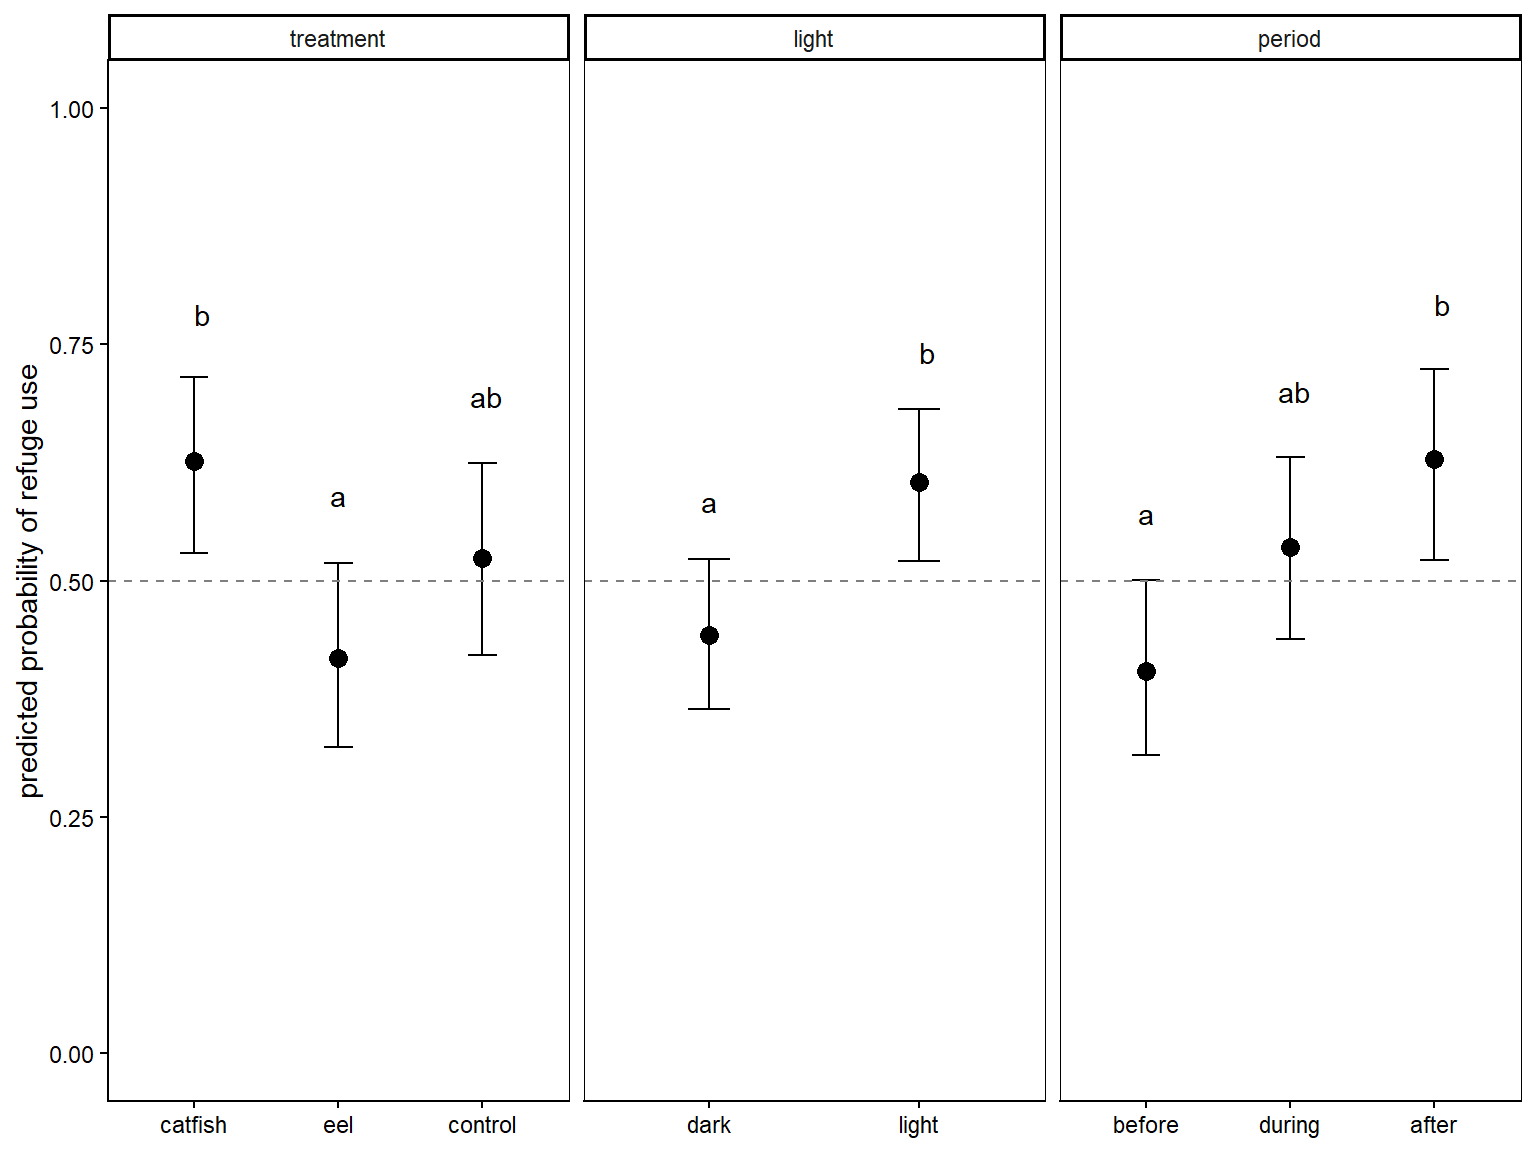
\includegraphics[keepaspectratio]{index_files/figure-latex/analysis-fig-emmeans-plot-output-1.png}}

}

\caption{\label{fig-emmeans-plot}Predicted marginal probabilities of
refuge use from the beta-binomial GLMM for each level of treatment,
light condition, and experimental period. Points represent
model-estimated marginal means averaged over other factors, with 95\%
confidence intervals shown as error bars. Different letters (a, b)
indicate statistically significant differences between groups within
each factor based on Tukey-adjusted pairwise comparisons. The dashed
line at 0.5 marks the threshold where kōura spend half their time in
refuge.}

\end{figure}%

\textsubscript{Source:
\href{https://OlivierRaven.github.io/https---github.com-OlivierRaven-NCE_Koura_catfish/analysis-preview.html\#cell-fig-emmeans-plot}{Analysis
Notebook}}

\begin{figure}[H]

\centering{

\pandocbounded{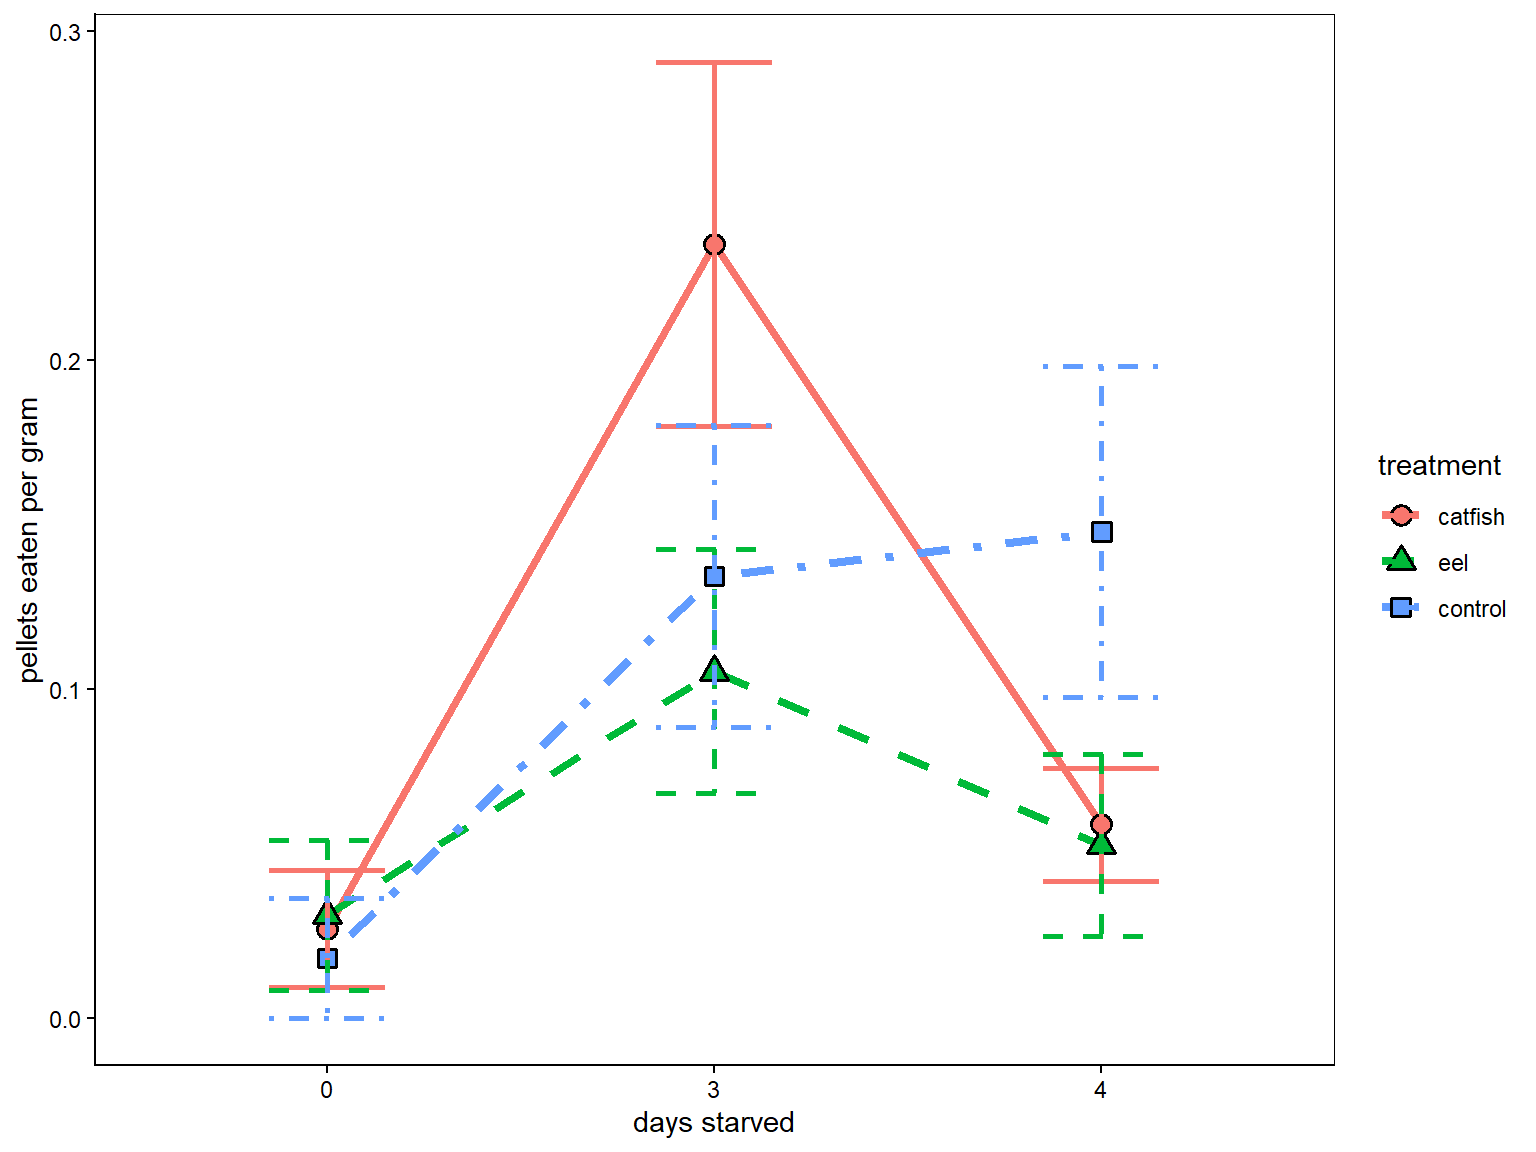
\includegraphics[keepaspectratio]{index_files/figure-latex/analysis-fig-feeding-plot-output-1.png}}

}

\caption{\label{fig-feeding-plot}Mean kōura feeding rate (pellets
consumed per gram body weight ± SE) across predator treatments (catfish,
eel, control) and starvation periods (0, 3, and 4 days). Points
represent treatment means and error bars show standard error.}

\end{figure}%

\textsubscript{Source:
\href{https://OlivierRaven.github.io/https---github.com-OlivierRaven-NCE_Koura_catfish/analysis-preview.html\#cell-fig-feeding-plot}{Analysis
Notebook}}

\section*{Supplementary information}\label{supplementary-information}
\addcontentsline{toc}{section}{Supplementary information}

\begin{table}

\caption{\label{tbl-s1-refuge-prop}Proportion of kōura observations
recorded in refuge across experimental treatments (catfish, eel,
control), light conditions (light, dark), and periods (before, during,
and after predator exposure). Combined rows summarise across all levels
of a given factor. Values represent the proportion of total observations
where kōura were located in the refuge.}

\centering{

\begin{verbatim}
Unable to display output for mime type(s): text/html
\end{verbatim}

}

\end{table}%

\textsubscript{Source:
\href{https://OlivierRaven.github.io/https---github.com-OlivierRaven-NCE_Koura_catfish/analysis-preview.html\#cell-tbl-s1-refuge-prop}{Analysis
Notebook}}

\begin{longtable}[]{@{}lrrrr@{}}

\caption{\label{tbl-s2-fixed-effects}Fixed effects of the beta-binomial
GLMM for kōura refuge use.}

\tabularnewline

\toprule\noalign{}
Term & Estimate & Std. Error & z value & p value \\
\midrule\noalign{}
\endhead
\bottomrule\noalign{}
\endlastfoot
(Intercept) & -0.058 & 0.282 & -0.206 & 0.837 \\
treatmentcatfish & 0.424 & 0.292 & 1.452 & 0.146 \\
treatmenteel & -0.427 & 0.294 & -1.452 & 0.147 \\
lightdark & -0.654 & 0.239 & -2.737 & 0.006 \\
periodduring & 0.530 & 0.282 & 1.881 & 0.060 \\
periodafter & 0.912 & 0.300 & 3.040 & 0.002 \\

\end{longtable}

\textsubscript{Source:
\href{https://OlivierRaven.github.io/https---github.com-OlivierRaven-NCE_Koura_catfish/analysis-preview.html\#cell-tbl-s2-fixed-effects}{Analysis
Notebook}}

\begin{longtable}[]{@{}
  >{\raggedright\arraybackslash}p{(\linewidth - 14\tabcolsep) * \real{0.2262}}
  >{\raggedleft\arraybackslash}p{(\linewidth - 14\tabcolsep) * \real{0.1429}}
  >{\raggedleft\arraybackslash}p{(\linewidth - 14\tabcolsep) * \real{0.0952}}
  >{\raggedleft\arraybackslash}p{(\linewidth - 14\tabcolsep) * \real{0.0714}}
  >{\raggedleft\arraybackslash}p{(\linewidth - 14\tabcolsep) * \real{0.0833}}
  >{\raggedleft\arraybackslash}p{(\linewidth - 14\tabcolsep) * \real{0.1071}}
  >{\raggedleft\arraybackslash}p{(\linewidth - 14\tabcolsep) * \real{0.1071}}
  >{\raggedright\arraybackslash}p{(\linewidth - 14\tabcolsep) * \real{0.1429}}@{}}

\caption{\label{tbl-s3-emmeans}Pairwise contrasts from the beta-binomial
GLMM for kōura refuge use. Odds ratios and p-values are shown for
treatment, light condition, and period comparisons. P-values are
Tukey-adjusted for multiple comparisons within each factor.}

\tabularnewline

\toprule\noalign{}
\begin{minipage}[b]{\linewidth}\raggedright
Contrast
\end{minipage} & \begin{minipage}[b]{\linewidth}\raggedleft
Odds ratio
\end{minipage} & \begin{minipage}[b]{\linewidth}\raggedleft
SE
\end{minipage} & \begin{minipage}[b]{\linewidth}\raggedleft
df
\end{minipage} & \begin{minipage}[b]{\linewidth}\raggedleft
Null
\end{minipage} & \begin{minipage}[b]{\linewidth}\raggedleft
z value
\end{minipage} & \begin{minipage}[b]{\linewidth}\raggedleft
p value
\end{minipage} & \begin{minipage}[b]{\linewidth}\raggedright
Factor
\end{minipage} \\
\midrule\noalign{}
\endhead
\bottomrule\noalign{}
\endlastfoot
control / catfish & 0.655 & 0.191 & Inf & 1 & -1.452 & 0.314 &
treatment \\
control / eel & 1.533 & 0.451 & Inf & 1 & 1.452 & 0.314 & treatment \\
catfish / eel & 2.341 & 0.681 & Inf & 1 & 2.924 & 0.010 & treatment \\
light / dark & 1.924 & 0.460 & Inf & 1 & 2.737 & 0.006 & light \\
before / during & 0.589 & 0.166 & Inf & 1 & -1.881 & 0.144 & period \\
before / after & 0.402 & 0.121 & Inf & 1 & -3.040 & 0.007 & period \\
during / after & 0.682 & 0.205 & Inf & 1 & -1.276 & 0.409 & period \\

\end{longtable}

\textsubscript{Source:
\href{https://OlivierRaven.github.io/https---github.com-OlivierRaven-NCE_Koura_catfish/analysis-preview.html\#cell-tbl-s3-emmeans}{Analysis
Notebook}}

\begin{longtable}[]{@{}lrrrr@{}}

\caption{\label{tbl-s4-feeding-anova}Type III ANOVA table for the linear
model of kōura feeding rate (pellets consumed per gram body weight).
Treatment, starvation period, and their interaction were included as
fixed effects.}

\tabularnewline

\toprule\noalign{}
Term & Sum Sq & Df & F value & p value \\
\midrule\noalign{}
\endhead
\bottomrule\noalign{}
\endlastfoot
(Intercept) & 0.004 & 1 & 0.640 & 0.429 \\
treatment & 0.000 & 2 & 0.032 & 0.968 \\
day\_starve & 0.132 & 2 & 9.571 & 0.000 \\
treatment:day\_starve & 0.062 & 4 & 2.241 & 0.082 \\
Residuals & 0.268 & 39 & NA & NA \\

\end{longtable}

\textsubscript{Source:
\href{https://OlivierRaven.github.io/https---github.com-OlivierRaven-NCE_Koura_catfish/analysis-preview.html\#cell-tbl-s4-feeding-anova}{Analysis
Notebook}}




\end{document}
